\documentclass[tikz,border=0pt]{standalone}
\usepackage{xcolor}
\usetikzlibrary{calc}
% Palette: Sam_Comm_final.png by eye, and the drones and raiders.
\definecolor{ink}{HTML}{3B2340}
\definecolor{sky}{HTML}{EFC46A}
\definecolor{skyhi}{HTML}{F5DA92}
\definecolor{skylow}{HTML}{E9B060}
\definecolor{cloud}{HTML}{F2D58A}
\definecolor{paper}{HTML}{FBEFD0}
\definecolor{cream}{HTML}{FFF6E0}
\definecolor{white}{HTML}{FFFFFF}
\definecolor{wallA}{HTML}{E88A73}
\definecolor{wallB}{HTML}{EE9F7E}
\definecolor{wallC}{HTML}{E47A7E}
\definecolor{wallD}{HTML}{F0B07E}
\definecolor{wallE}{HTML}{D9765F}
\definecolor{wallF}{HTML}{E99A8A}
\definecolor{greenA}{HTML}{8DBB7E}
\definecolor{greenB}{HTML}{6FA77A}
\definecolor{greenC}{HTML}{A9C97F}
\definecolor{greenD}{HTML}{5E9C6A}
\definecolor{greenE}{HTML}{4A8060}
\definecolor{sage}{HTML}{9DB98A}
\definecolor{sagedark}{HTML}{6F8F66}
\definecolor{sagelight}{HTML}{C2D6A6}
\definecolor{window}{HTML}{F6E7A0}
\definecolor{windark}{HTML}{8C5A64}
\definecolor{metal}{HTML}{8D9A93}
\definecolor{metaldark}{HTML}{5E6B66}
\definecolor{metallight}{HTML}{B9C4BC}
\definecolor{wood}{HTML}{B9835A}
\definecolor{wooddark}{HTML}{8C5A3C}
\definecolor{woodlight}{HTML}{D9A66F}
\definecolor{stone}{HTML}{E7C9A0}
\definecolor{stonedark}{HTML}{C9A47E}
\definecolor{concrete}{HTML}{D8C3A4}
\definecolor{concretedark}{HTML}{B8A084}
\definecolor{asphalt}{HTML}{8E7A86}
\definecolor{asphaltdark}{HTML}{6E5C68}
\definecolor{roadline}{HTML}{F6E7A0}
\definecolor{kerb}{HTML}{D8B48C}
\definecolor{red}{HTML}{E0483E}
\definecolor{redlight}{HTML}{F27A6A}
\definecolor{gold}{HTML}{FFB000}
\definecolor{goldlight}{HTML}{FFD54F}
\definecolor{teal}{HTML}{4FA3A0}
\definecolor{tealdark}{HTML}{3C8582}
\definecolor{magenta}{HTML}{FF2E88}
\definecolor{cyan}{HTML}{13CFE3}
\definecolor{violet}{HTML}{8A5BD6}
\definecolor{orange}{HTML}{F2803A}
\definecolor{pink}{HTML}{F48FB1}
\definecolor{glow}{HTML}{4FE6E0}
\definecolor{glowhi}{HTML}{C8FFF9}
\definecolor{hot}{HTML}{FF6A1A}
\definecolor{hothi}{HTML}{FFD07A}
\definecolor{armour}{HTML}{7E7A86}
\definecolor{armourdark}{HTML}{5A5466}
\definecolor{armourlight}{HTML}{A8A2B0}
\definecolor{wasp}{HTML}{E0A82E}
\definecolor{waspdark}{HTML}{B07E1A}
\definecolor{moth}{HTML}{F2E6C8}
\definecolor{mothdark}{HTML}{D2C09A}
\definecolor{hornet}{HTML}{3C8582}
\definecolor{hornetdark}{HTML}{2C6260}
\definecolor{warden}{HTML}{E47A7E}
\definecolor{wardendark}{HTML}{B85A62}
\definecolor{tick}{HTML}{8DBB7E}
\definecolor{tickdark}{HTML}{5E8A5A}
\definecolor{strider}{HTML}{D9765F}
\definecolor{striderdark}{HTML}{A8543F}
\definecolor{jacket}{HTML}{6FA77A}
\definecolor{jacketb}{HTML}{4FA3A0}
\definecolor{jacketc}{HTML}{E88A73}
\definecolor{jacketd}{HTML}{F0B07E}
\definecolor{skin}{HTML}{F2C49A}
\definecolor{skinb}{HTML}{C98C6A}
\definecolor{skinc}{HTML}{8C5A3C}
\definecolor{hair}{HTML}{3B2340}
\definecolor{goo}{HTML}{B6E35A}
\definecolor{goodark}{HTML}{7FB23A}
\newcommand{\Ink}{1.8pt}
\tikzset{inked/.style={draw=ink, line width=\Ink, line join=round, line cap=round}}
\begin{document}
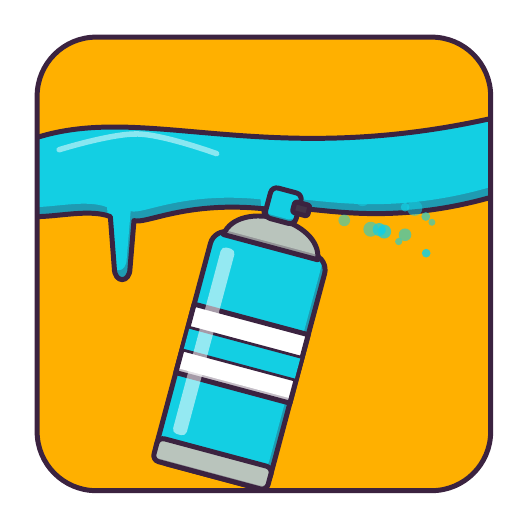
\begin{tikzpicture}
\clip (0,0) rectangle (6,6);
\fill[gold] [rounded corners=0.75cm] (0.12,0.12) rectangle (5.88,5.88);
\begin{scope}\clip [rounded corners=0.75cm] (0.12,0.12) rectangle (5.88,5.88);
\begin{scope}\clip (0.1,4.6) .. controls (1.5,5.05) and (3.0,4.2) .. (5.9,4.85) -- (5.9,3.85) .. controls (4.5,3.45) and (3.6,3.75) .. (3.3,3.7) -- (3.25,3.15) .. controls (3.25,3.0) and (3.05,3.0) .. (3.05,3.15) -- (3.0,3.7) .. controls (2.0,3.8) and (1.5,3.5) .. (1.35,3.55) -- (1.3,2.95) .. controls (1.3,2.75) and (1.1,2.75) .. (1.1,2.95) -- (1.05,3.6) .. controls (0.8,3.7) and (0.4,3.6) .. (0.1,3.6) -- cycle;
\fill[cyan!70!ink] (0.1,4.6) .. controls (1.5,5.05) and (3.0,4.2) .. (5.9,4.85) -- (5.9,3.85) .. controls (4.5,3.45) and (3.6,3.75) .. (3.3,3.7) -- (3.25,3.15) .. controls (3.25,3.0) and (3.05,3.0) .. (3.05,3.15) -- (3.0,3.7) .. controls (2.0,3.8) and (1.5,3.5) .. (1.35,3.55) -- (1.3,2.95) .. controls (1.3,2.75) and (1.1,2.75) .. (1.1,2.95) -- (1.05,3.6) .. controls (0.8,3.7) and (0.4,3.6) .. (0.1,3.6) -- cycle;
\fill[cyan, shift={(-0.042,0.12)}] (0.1,4.6) .. controls (1.5,5.05) and (3.0,4.2) .. (5.9,4.85) -- (5.9,3.85) .. controls (4.5,3.45) and (3.6,3.75) .. (3.3,3.7) -- (3.25,3.15) .. controls (3.25,3.0) and (3.05,3.0) .. (3.05,3.15) -- (3.0,3.7) .. controls (2.0,3.8) and (1.5,3.5) .. (1.35,3.55) -- (1.3,2.95) .. controls (1.3,2.75) and (1.1,2.75) .. (1.1,2.95) -- (1.05,3.6) .. controls (0.8,3.7) and (0.4,3.6) .. (0.1,3.6) -- cycle;
\end{scope}
\draw[inked] (0.1,4.6) .. controls (1.5,5.05) and (3.0,4.2) .. (5.9,4.85) -- (5.9,3.85) .. controls (4.5,3.45) and (3.6,3.75) .. (3.3,3.7) -- (3.25,3.15) .. controls (3.25,3.0) and (3.05,3.0) .. (3.05,3.15) -- (3.0,3.7) .. controls (2.0,3.8) and (1.5,3.5) .. (1.35,3.55) -- (1.3,2.95) .. controls (1.3,2.75) and (1.1,2.75) .. (1.1,2.95) -- (1.05,3.6) .. controls (0.8,3.7) and (0.4,3.6) .. (0.1,3.6) -- cycle;
\draw[white, line width=2pt, line cap=round, line join=round, opacity=0.5] plot[smooth, tension=0.6] coordinates {(0.4,4.45) (1.4,4.65) (2.4,4.4)};
\begin{scope}[shift={(2.8,2.15)}, rotate=-15, xscale=1, yscale=1]
\begin{scope}\clip[rounded corners=0.2cm] (-0.75,-1.9) rectangle (0.75,1.15);
\fill[cyan!70!ink,rounded corners=0.2cm] (-0.75,-1.9) rectangle (0.75,1.15);
\fill[cyan,rounded corners=0.2cm, shift={(-0.063,0.18)}] (-0.75,-1.9) rectangle (0.75,1.15);
\end{scope}
\draw[inked,rounded corners=0.2cm] (-0.75,-1.9) rectangle (0.75,1.15);
\begin{scope}\clip (-0.75,-0.75) rectangle (0.75,0.15);
\fill[white!70!ink] (-0.75,-0.75) rectangle (0.75,0.15);
\fill[white, shift={(-0.021,0.06)}] (-0.75,-0.75) rectangle (0.75,0.15);
\end{scope}
\draw[inked] (-0.75,-0.75) rectangle (0.75,0.15);
\fill[cyan] (-0.73,-0.45) rectangle (0.73,-0.15);
\draw[ink, line width=1pt, line cap=round] (-0.73,-0.45) -- (0.73,-0.45);
\draw[ink, line width=1pt, line cap=round] (-0.73,-0.15) -- (0.73,-0.15);
\begin{scope}\clip (-0.62,1.1) .. controls (-0.55,1.6) and (0.55,1.6) .. (0.62,1.1) -- cycle;
\fill[metallight!70!ink] (-0.62,1.1) .. controls (-0.55,1.6) and (0.55,1.6) .. (0.62,1.1) -- cycle;
\fill[metallight, shift={(-0.021,0.06)}] (-0.62,1.1) .. controls (-0.55,1.6) and (0.55,1.6) .. (0.62,1.1) -- cycle;
\end{scope}
\draw[inked] (-0.62,1.1) .. controls (-0.55,1.6) and (0.55,1.6) .. (0.62,1.1) -- cycle;
\begin{scope}\clip[rounded corners=0.08cm] (-0.18,1.45) rectangle (0.22,1.85);
\fill[cyan!70!ink,rounded corners=0.08cm] (-0.18,1.45) rectangle (0.22,1.85);
\fill[cyan,rounded corners=0.08cm, shift={(-0.017,0.05)}] (-0.18,1.45) rectangle (0.22,1.85);
\end{scope}
\draw[inked,rounded corners=0.08cm] (-0.18,1.45) rectangle (0.22,1.85);
\begin{scope}\clip[rounded corners=0.03cm] (0.15,1.6) rectangle (0.35,1.74);
\fill[ink!78!metaldark!70!ink,rounded corners=0.03cm] (0.15,1.6) rectangle (0.35,1.74);
\fill[ink!78!metaldark,rounded corners=0.03cm, shift={(0,0)}] (0.15,1.6) rectangle (0.35,1.74);
\end{scope}
\draw[inked,rounded corners=0.03cm] (0.15,1.6) rectangle (0.35,1.74);
\begin{scope}\clip[rounded corners=0.08cm] (-0.75,-1.9) rectangle (0.75,-1.6);
\fill[metallight!70!ink,rounded corners=0.08cm] (-0.75,-1.9) rectangle (0.75,-1.6);
\fill[metallight,rounded corners=0.08cm, shift={(-0.014,0.04)}] (-0.75,-1.9) rectangle (0.75,-1.6);
\end{scope}
\draw[inked,rounded corners=0.08cm] (-0.75,-1.9) rectangle (0.75,-1.6);
\fill[white, opacity=0.55, rounded corners=0.06cm] (-0.6,-1.5) rectangle (-0.42,0.95);
\fill[cyan, opacity=0.7] (0.3,-1.1) circle (0.1) (0.45,-1.35) circle (0.06);
\end{scope}
\fill[cyan, opacity=0.748] (4.528,3.41) circle (0.088);
\fill[cyan, opacity=0.528] (4.021,3.553) circle (0.074);
\fill[cyan, opacity=0.72] (4.793,3.72) circle (0.055);
\fill[cyan, opacity=0.603] (4.792,3.37) circle (0.08);
\fill[cyan, opacity=0.505] (4.915,3.708) circle (0.098);
\fill[cyan, opacity=0.631] (5.056,3.602) circle (0.056);
\fill[cyan, opacity=0.624] (4.712,3.284) circle (0.046);
\fill[cyan, opacity=0.598] (4.949,4.277) circle (0.094);
\fill[cyan, opacity=0.842] (5.061,3.136) circle (0.055);
\fill[cyan, opacity=0.841] (4.502,3.424) circle (0.043);
\fill[cyan, opacity=0.862] (4.988,4.282) circle (0.082);
\fill[cyan, opacity=0.624] (4.396,3.854) circle (0.05);
\fill[cyan, opacity=0.584] (5.134,3.528) circle (0.044);
\fill[cyan, opacity=0.747] (4.465,3.436) circle (0.083);
\fill[cyan, opacity=0.548] (4.251,3.821) circle (0.088);
\fill[cyan, opacity=0.899] (4.958,4.3) circle (0.089);
\fill[cyan, opacity=0.557] (4.358,3.44) circle (0.095);
\fill[cyan, opacity=0.78] (4.614,3.884) circle (0.097);
\end{scope}
\draw[inked] [rounded corners=0.75cm] (0.12,0.12) rectangle (5.88,5.88);
\end{tikzpicture}
\end{document}
